\documentclass[11pt,a4paper]{article}

\usepackage[margin=2.5cm]{geometry}
\usepackage{amsmath,amssymb,amsthm}
\usepackage{booktabs}
\usepackage{graphicx}
\usepackage{tikz}
\usetikzlibrary{arrows.meta,positioning}
\usepackage[T1]{fontenc}
\usepackage[utf8]{inputenc}
\usepackage[expansion=false]{microtype}
\usepackage{array}
\usepackage{algorithm}
\usepackage{algpseudocode}
\usepackage{hyperref}

\theoremstyle{definition}
\newtheorem{definition}{Definition}
\theoremstyle{plain}
\newtheorem{theorem}{Theorem}
\newtheorem{lemma}[theorem]{Lemma}
\newtheorem{proposition}[theorem]{Proposition}
\newtheorem{corollary}[theorem]{Corollary}
\theoremstyle{remark}
\newtheorem{fact}{Fact}
\newtheorem{remark}{Remark}
\newtheorem{example}{Example}

\newcommand{\cov}{\operatorname{cov}}
\newcommand{\orig}{\operatorname{orig}}
\newcommand{\name}{\operatorname{name}}
\newcommand{\isize}{\operatorname{isize}}
\newcommand{\lcp}{\operatorname{lcp}}
\newcommand{\Feas}{\mathcal{F}}
\newcommand{\Links}{\mathcal{K}}
\newcommand{\Names}{\mathcal{N}}
\newcommand{\pref}{\pi}
\newcommand{\KEEP}{\textnormal{\textsc{Keep}}}
\newcommand{\COMP}{\textnormal{\textsc{Compress}}}

\algrenewcommand\algorithmicrequire{\textbf{Input:}}
\algrenewcommand\algorithmicensure{\textbf{Output:}}

\title{\texttt{tree-dp}: the preference-forest dynamic program\\
for differential compression of the gapped suffix array}
\author{}
\date{}

\begin{document}
\maketitle

\begin{abstract}
\noindent
\texttt{tree-dp} compresses a gapped suffix array by choosing, for each
gapped $k$-mer name, at most one \emph{link} that replaces a run of
stored positions by a pointer plus a shift. It does so in five stages:
enumerate a pruned candidate universe; let every name nominate a single
\emph{preferred} link; observe that the resulting ``who sources from
whom'' graph has out-degree at most one and is therefore a
\emph{pseudoforest}; delete one edge per cycle to obtain a forest; and
solve the restricted problem on that forest \emph{exactly} by a
two-state \KEEP/\COMP{} dynamic program. A materialization pass, an
availability greedy over the names the forest never reached, and a
shared unpin/retarget fixed point complete the algorithm. This note is
the definitive description of that base algorithm. It states and proves
the pseudoforest property that makes the DP possible; it isolates the
three places where optimality is lost (one link per name, one parent per
name, and an arbitrarily chosen cut edge); and it demonstrates the third
loss on a family of $24$ instances that are pairwise \emph{isomorphic}
as optimization problems --- identical interval sizes and identical
$15$-link universes under a relabelling, and optimum $|C| = 11$
throughout --- on which \texttt{tree-dp} returns $11$ for eight of them
and $13$ for the other sixteen, while every order-independent algorithm
in the family returns one value for all $24$. The difference is nothing
but the arithmetic order of four $k$-mer names. Everything numerical
here was produced by the committed binaries at \texttt{7f9127b}.
\end{abstract}

\tableofcontents

\section{Scope, and how this note relates to the others}
\label{sec:scope}

Three documents in \texttt{doc/} now describe overlapping parts of the
same pipeline.

\begin{itemize}
\item \texttt{dep\_order\_walkthrough} builds the gapped suffix array
  from scratch on a three-fold repeat of \texttt{GCCTTTAAAG}, defines
  links, and walks through \texttt{greedy}, \texttt{dep-order} and
  (in \S6) an early version of \texttt{tree-dp}. It is the right place
  to learn what a gapped suffix array \emph{is}.
\item \texttt{tree\_dp3} formalizes the optimization problem, proves it
  is a set-packing problem with two \emph{pairwise} constraints and no
  acyclicity requirement, and builds the exact cluster-local
  re-optimization \texttt{tree-dp3} on top of that.
\item This note treats \texttt{tree-dp} itself in full.
\end{itemize}

We take the notation of \texttt{tree\_dp3} \S1 as given: a link is a
tuple $k = (c_k, a_k, S_k, T_k)$ with target name $c_k$, shift $a_k$,
source ranks $S_k$ and covered ranks $T_k$; validity conditions
(V1)--(V3); feasibility conditions (F1) ``one link per name'' and (F2)
``a chosen link's source ranks are all kept''; and the objective
\[
  |C|(X) \;=\; m - \cov(X),
  \qquad
  \cov(X) = \sum_{k \in X} \cov(k),
  \qquad
  \cov(k) = |T_k| = |S_k|.
\]
Section~\ref{sec:setup} recalls just enough of this to be readable
standalone. Where \texttt{tree\_dp3} already proves something we cite it
rather than repeat it.

The reader who wants only the algorithm can read
\S\ref{sec:enumerate}--\S\ref{sec:phase2}; the reader who wants to see
it run should go to \S\ref{sec:example}.

A note on provenance. All measurements below come from a clean build of
the tree at commit \texttt{7f9127b} (\emph{Add the tree-dp3 writeup}),
extracted with \texttt{git archive} into a scratch directory and built
with the repository \texttt{Makefile}. This matters because the working
tree carried unrelated uncommitted changes at the time of writing.

\section{Setup}
\label{sec:setup}

Fix a binary shape $S$ of span $s$ over a text $T[0..n)$. Every position
$p$ carries a gapped $k$-mer \emph{name}, the $w$ characters selected by
the care positions of $S$ placed at $p$. The DisLex transform groups the
names by residue class $p \bmod s$ and the suffix array of the resulting
lextext is the \textbf{gapped suffix array} (GSA), with $m = n+1$ ranks.
We write $\orig(r)$ for the text position of rank $r$ and $\name(r)$ for
its gapped $k$-mer.

Because the GSA is sorted by gapped suffix, the ranks carrying a fixed
name $c$ are contiguous: they form the \textbf{interval}
$I_c = [\ell_c, r_c)$ of size $\isize(c) = r_c - \ell_c$. The intervals
partition $\{0,\dots,m-1\}$. Let $\Names$ be the set of names with
$\isize(c) > 1$; singleton intervals are never compressed.

\begin{definition}[Link]
\label{def:link}
A \textbf{link} $k$ with target name $c$, shift $a \ge 1$, source run
$S_k = [s_{\mathrm{lo}}, s_{\mathrm{hi}})$ and covered set $T_k$ is
\emph{valid} when
\begin{description}
\item[(V1)] shifting the $j$-th source rank by $a$ windows gives the
  $j$-th covered rank, that is
  $\orig(T_k[j]) = \orig(S_k[j]) + a\cdot s$, and every covered rank
  carries the name $c$;
\item[(V2)] $S_k \cap T_k = \emptyset$;
\item[(V3)] $\cov(k) = |T_k| = |S_k| \ge \kappa$, where $\kappa = 3$ is
  \texttt{kMinCoverage}.
\end{description}
\end{definition}

Accepting a link means: drop every rank of $T_k$ from the compressed
array $C$, and store in the hash entry for $c$ an
$H_{\mathrm{offset}} = (\mathit{pos}, a, \mathit{num})$ recording where
$S_k$ starts in $C$, the shift, and how many positions it regenerates.
The ranks of $I_c$ that no link covers are stored literally and pointed
at by $H_{\mathrm{rest}}$. Decoding is a single addition per covered
position and never recurses --- a fact that \texttt{tree\_dp3}
(Proposition~2) shows removes any acyclicity requirement from the
problem, and that we will lean on in \S\ref{sec:phase2}.

A set $X$ of valid links is \textbf{feasible} when every pair
$k \ne k'$ in $X$ satisfies

\begin{description}
\item[(F1)] $c_k \ne c_{k'}$ (one $H_{\mathrm{offset}}$ per hash entry),
  and
\item[(F2)] $S_k \cap T_{k'} = \emptyset$ (a source must be physically
  present in $C$).
\end{description}

Since $|C|(X) = m - \cov(X)$, minimizing $|C|$ is maximizing total
coverage subject to (F1) and (F2). Throughout, $a_{\max}$ denotes
\texttt{--max-add} (default $8$).

\section{Phase 0: candidate enumeration}
\label{sec:enumerate}

The link universe of \S\ref{sec:setup} is far too large to hand to a
heuristic: it has $\Theta(m \cdot a_{\max})$ maximal runs and, if
sub-runs are counted, $\Theta(m \cdot a_{\max} \cdot L)$ links for runs
of length $L$. \texttt{enumerate\_candidates\_} produces a pruned view of
it, one interval at a time. This pruned view is what every heuristic
sees; the full universe is enumerated only by
\texttt{enumerate\_all\_links\_}, which feeds the ILP baseline and
therefore gives a genuine lower bound on all of them.

\subsection{The scan}

Fix a name $c$ with interval $I_c = [\ell, r)$ and a shift $a$. For each
rank $t \in I_c$ the routine asks: is there a rank $u$ whose text
position is exactly $\orig(t) - a\cdot s$, in the same residue class?
This is \texttt{pred\_lexpos\_}, a constant-time lookup in the lextext.
The surviving pairs $(u,t)$ are sorted by $u$, giving a list
\[
  \mathit{pr} = \bigl[(u_1,t_1), (u_2,t_2), \dots\bigr],
  \qquad u_1 < u_2 < \cdots .
\]
Each pair is a one-position link; a candidate is a \emph{run} of
consecutive pairs.

The run is cut at two kinds of boundary. The first is obvious: $u$ must
advance by exactly one rank, $u_{j} = u_{j-1} + 1$. The second is the
interesting one:
\[
  \lcp[u_j] \;\ge\; a+1 .
\]

\begin{remark}[Why $\lcp \ge a+1$]
\label{rem:lcp}
Adjacent ranks $u_{j-1}, u_j$ agreeing in their first $a+1$ gapped
symbols is exactly the condition under which shifting both forward by
$a$ windows lands them in the \emph{same} target interval and preserves
their relative order. Weaker agreement can still yield valid links ---
\texttt{enumerate\_all\_links\_} emits them --- but the resulting source
runs are not lcp-intervals and the enumeration loses the property that
each run is described by a single contiguous rank range. The heuristics
accept the loss: $\lcp \ge a+1$ is a pruning rule, not a correctness
one.
\end{remark}

A run of length $\cov$ shorter than $\kappa = 3$ is discarded outright
(\texttt{emit\_run\_} returns immediately). This floor is not a
tuning parameter that happens to be set to $3$; it is the point below
which a link stops paying for itself, because the hash entry that stores
it costs space too.

\begin{remark}[The floor is visible in the older walkthrough]
On the walkthrough's running example $T = (\mathtt{GCCTTTAAAG})^3$ with
$S = \mathtt{\#.\#}$, the names \texttt{CT} and \texttt{GC} were
described as preferring each other with coverage $2$. At
\texttt{7f9127b} those links are never enumerated at all, and
\texttt{CT} and \texttt{GC} have \emph{no} candidates whatsoever. See
\S\ref{sec:continuity}.
\end{remark}

\subsection{Availability}

\texttt{enumerate\_candidates\_} takes a flag \texttt{require\_avail}.
When set, a candidate is emitted only if
\begin{itemize}
\item every rank of its source run is still kept
  (\texttt{run\_kept\_}), which is (F2); and
\item no rank it covers is already removed, and no rank it covers is
  \emph{pinned} --- i.e.\ is currently serving as a source rank for some
  accepted link.
\end{itemize}
The pin counter \texttt{pin\_count\_} is what enforces (F2) dynamically.
Preferences (\S\ref{sec:pref}) are computed with
\texttt{require\_avail=false}: they are a static, structural notion,
computed once before anything has been accepted, and cached for reuse by
the leftover pass and Phase~II.

\subsection{Intra-interval links}
\label{sec:intra}

Historically a source run overlapping $I_c$ was rejected: a link was
required to source from a \emph{different} name's interval. That rule is
stronger than necessary. What (V2) actually demands is only
$S_k \cap T_k = \emptyset$: the source must not contain any of the ranks
the link itself deletes. A run that overlaps $I_c$ but avoids its own
covered ranks decodes perfectly well.

When the source run of the scan lands inside $I_c$,
\texttt{emit\_intra\_runs\_} therefore does not discard it; it splits it
into maximal sub-runs that are free of the self-conflict. In run-relative
coordinates, position $t$ of the run covers rank $u$; the window
$[p,q)$ is bad exactly when it contains both $t$ and $u$ for some pair.
The routine precomputes, for each right endpoint $b$, the smallest window
start that still traps a pair ending at $b$, then sweeps $q$ with a
monotone left pointer $p$, emitting a window whenever it cannot be grown
to the right without moving $p$. Monotonicity of $p$ means no emitted
window contains another, so the output is the antichain of maximal
conflict-free sub-runs, computed in linear time in the run length.

The sub-run splitting is what makes intra-interval links useful rather
than merely legal: the whole run is almost always self-conflicting,
while its halves are not.

\begin{example}[Intra-interval links are not a corner case]
\label{ex:a16}
Take $T = \mathtt{A}^{16}$, $S = \mathtt{\#.\#}$, so $m = 17$. There are
three names: $\mathtt{\$\$}$ (one rank), $\mathtt{A\$}$ (two ranks) and
$\mathtt{AA}$ (fourteen ranks, $I_{\mathtt{AA}} = [3,17)$). Only
$\mathtt{AA}$ is compressible, and the only place a source run can
possibly come from is $I_{\mathtt{AA}}$ itself. Then
\[
  \texttt{tree-dp} \Rightarrow |C| = 11,
  \qquad
  \texttt{GCSA\_INTRA\_LINKS=0} \Rightarrow |C| = 17 .
\]
With intra-interval links disabled the instance is incompressible; with
them enabled \texttt{tree-dp} attains $|C| = 11$, which the ILP
baseline confirms is optimal. This example returns in
\S\ref{sec:dp:intra}, where it exposes something less comfortable.
\end{example}

\subsection{The role of \texttt{--max-add}}

The scan runs $a = 1, \dots, a_{\max}$. Raising $a_{\max}$ strictly
enlarges every candidate list, so it can only help a hypothetical
optimizer --- and, empirically, it does help the exact one: at
$a_{\max} = 16$, \texttt{tree-dp3} improves suite-wide $|C|$ by nearly
$16\,\%$ over $a_{\max} = 8$, whereas \texttt{tree-dp} barely moves
(\S\ref{sec:empirical}). For \texttt{tree-dp} the extra candidates are
mostly invisible, because each name still contributes exactly one
preferred link to the forest and the preferred link rarely changes: a
larger shift is chosen only to break a coverage tie. The candidate
universe is not \texttt{tree-dp}'s binding constraint; the forest is.

\section{Preference selection and the pseudoforest}
\label{sec:pref}

\subsection{Preferences}

For every name $c$ with $\isize(c) > 2$, \texttt{tree-dp} computes the
full static candidate list $\hat\Links_c$ and records a single
\textbf{preferred} link
\[
  \pref(c) \;=\; \arg\max_{k \in \hat\Links_c} \ \bigl(\cov(k),\ a_k\bigr)
\]
in lexicographic order: maximum coverage, ties broken towards the
\emph{larger} shift (\texttt{pick\_best\_}). If the best candidate has
coverage below $\kappa$ --- or if the list is empty --- the name has no
preference. Note the threshold $\isize(c) > 2$ rather than $> 1$: an
interval of size $2$ cannot host a link of coverage $3$ anyway.

The tie-break towards larger $a$ looks cosmetic. It is not: it decides
which \emph{name} a preference points at, and hence the shape of the
graph built next. We will see it change the answer in
\S\ref{sec:example:cand}.

\subsection{The preference graph}

Draw a directed edge $c \to w$ whenever the source run of $\pref(c)$
lies inside $I_w$. The following is the structural fact on which the
entire algorithm rests.

\begin{proposition}[Out-degree at most one]
\label{prop:outdeg}
Each name has at most one outgoing preference edge, and the target $w$
is well defined.
\end{proposition}

\begin{proof}
A name has at most one preferred link, so at most one edge. For
well-definedness we must show the source run
$S = [s_{\mathrm{lo}}, s_{\mathrm{hi}})$ of a candidate lies inside a
single interval. By construction the run was cut wherever
$\lcp[u] < a+1$, so all ranks of $S$ agree in their first $a+1$ gapped
symbols. Since $a \ge 1$, they agree in at least their first $2$
symbols, hence certainly in their first symbol, which is precisely the
name. As intervals are the maximal blocks of constant first symbol,
$S \subseteq I_w$ for exactly one $w$.
\end{proof}

\begin{corollary}[Pseudoforest]
\label{cor:pseudoforest}
The preference graph, viewed as an undirected graph, is a
\textbf{pseudoforest}: every connected component contains at most one
cycle.
\end{corollary}

\begin{proof}
A component with $\nu$ vertices has at most $\nu$ edges, since each
vertex contributes at most one out-edge. A connected graph on $\nu$
vertices with at most $\nu$ edges has cyclomatic number at most $1$.
\end{proof}

This is the whole reason a dynamic program is available. An arbitrary
``$c$ can source from $w$'' relation is a dense digraph on $\Names$ and
optimizing over it is the set-packing problem of
\texttt{tree\_dp3}~\S1.4, which is NP-hard in general. Restricting each
name to one preferred link collapses that digraph to a functional graph,
and functional graphs are one edge-deletion per component away from
forests, where dynamic programming is routine.

Two degenerate cases deserve names.

\begin{itemize}
\item \textbf{Self-loops.} If $\pref(c)$ is an intra-interval link
  (\S\ref{sec:intra}) then $w = c$ and the edge is a self-loop.
\item \textbf{Dangling sources.} If $I_w$ is a singleton it is not in
  $\Names$ and the edge points at a vertex the algorithm does not model;
  the edge is dropped (\texttt{by\_name.count(s)}).
\end{itemize}

\section{Cycle breaking}
\label{sec:cyclebreak}

The DP needs a forest, so one edge per cycle must go. The
implementation does this while installing edges, in a single pass:

\begin{algorithm}[t]
\caption{Forest construction from preferences}
\label{alg:forest}
\begin{algorithmic}[1]
\Require preferences $\pref(\cdot)$, intervals by name
\Ensure a parent map inducing a forest
\State $\mathrm{parent} \gets \emptyset$
\ForAll{names $c$ with a preference, \textbf{in ascending name code order}}
  \State $w \gets$ the name whose interval contains the source of $\pref(c)$
  \If{$\cov(\pref(c)) < \kappa$} \textbf{continue} \EndIf
  \If{$w = c$} \textbf{continue}
    \Comment{intra-interval link: self-loop}
  \EndIf
  \If{$\isize(w) \le 1$} \textbf{continue}
    \Comment{source in a singleton interval}
  \EndIf
  \If{\Call{HasAncestor}{$w$, $c$}} \textbf{continue}
    \Comment{would close a cycle: \emph{discard}}
  \EndIf
  \State $\mathrm{parent}[c] \gets w$
\EndFor
\end{algorithmic}
\end{algorithm}

\texttt{HasAncestor}$(w,c)$ walks the parent chain up from $w$ and
reports whether it meets $c$. Since the partial structure is always a
forest, the walk terminates and costs $O(\mathrm{depth})$.

Two properties of this loop matter.

\begin{fact}[The cut edge is chosen by name order, not by value]
\label{fact:order}
For a cycle $c_1 \to c_2 \to \cdots \to c_\nu \to c_1$, the edge
discarded is the out-edge of whichever cycle vertex the loop visits
last. The loop visits names in ascending arithmetic code order --- the
integer encoding of the $k$-mer, i.e.\ essentially alphabetical order of
the gapped $k$-mer string. Nothing about the coverages, shifts or
interval sizes of the cycle's edges enters the decision.
\end{fact}

The comment in the source calls the iteration order ``deterministic
\dots so parallel pref build does not change which cycle-breaking edges
survive''. That is true and worth having --- the result is reproducible
--- but reproducibility is not optimality. A cycle of $\nu$ edges offers
$\nu$ distinct forests and the algorithm takes the one indexed by the
alphabet.

\begin{fact}[This is where the loss is]
\label{fact:loss}
\texttt{tree-dp} is exact on the model it constructs
(Theorem~\ref{thm:dpexact}). Optimality can therefore only be lost when
the model is built. There are exactly three lossy steps:
\begin{enumerate}
\item each name is restricted to its \emph{single} preferred link
  (\S\ref{sec:pref});
\item each name is restricted to its \emph{single} parent, so a name
  that could serve as source for several dependents' second-choice
  links cannot;
\item one edge per cycle is deleted by Fact~\ref{fact:order}.
\end{enumerate}
\end{fact}

Section~\ref{sec:twin} exhibits the third loss in the sharpest form
available: twenty-four instances that are all the same optimization
problem up to renaming, on which \texttt{tree-dp} returns two different
answers depending only on the alphabet. Section~\ref{sec:ce} recalls a
second, smaller instance where the same restriction bites and where ---
unlike in \S\ref{sec:twin} --- no later pass can repair it.

\section{\texorpdfstring{The \KEEP/\COMP{} dynamic program}{The KEEP/COMPRESS dynamic program}}
\label{sec:dp}

\subsection{States and recurrence}

Each forest node $v$ is a name with interval size $\isize(v)$ and (if it
has a preference) a candidate $\pref(v)$ of coverage $\cov(\pref(v))$
whose source lies in $\mathrm{parent}(v)$'s interval. The DP decides,
for each $v$, whether to
\begin{description}
\item[\KEEP] store all $\isize(v)$ ranks of $I_v$ literally, or
\item[\COMP] accept $\pref(v)$, storing $\isize(v) - \cov(\pref(v))$
  ranks.
\end{description}
The two decisions interact along forest edges in one direction only. If
$v$ compresses, its source ranks lie in $I_{\mathrm{parent}(v)}$ and must
survive, which by (F2) forbids \emph{every child of $v$} from covering
them. The implementation takes the conservative reading: a compressing
node forbids its children from compressing at all. This is what the
second state records.

\begin{definition}[DP states]
$\mathrm{DP}(v, \mathit{src\_ok})$ is the minimum number of stored ranks
in the subtree of $v$, where $\mathit{src\_ok} = \mathsf{true}$ means
$v$ is still allowed to accept $\pref(v)$.
\end{definition}

\begin{align}
  \mathrm{DP}(v,\mathsf{true}) &= \min\Bigl(
    \underbrace{\isize(v) + \!\!\sum_{w \in \mathrm{ch}(v)}\!\!
      \mathrm{DP}(w,\mathsf{true})}_{\KEEP},\;
    \underbrace{\isize(v) - \cov(\pref(v)) + \!\!\sum_{w \in \mathrm{ch}(v)}\!\!
      \mathrm{DP}(w,\mathsf{false})}_{\COMP}
  \Bigr),
  \label{eq:dptrue}\\[2pt]
  \mathrm{DP}(v,\mathsf{false}) &= \isize(v) + \!\!\sum_{w \in \mathrm{ch}(v)}\!\!
      \mathrm{DP}(w,\mathsf{true}).
  \label{eq:dpfalse}
\end{align}

The \COMP{} branch is available only when $\mathit{src\_ok}$ holds and
$\cov(\pref(v)) \ge \kappa$. Ties go to \KEEP{} (the code takes \COMP{}
only on \emph{strict} improvement), which is the right default: keeping
a hub free leaves options open for the leftover pass and Phase~II.

\subsection{The root rule}

A root has no parent inside the forest, so the source of its preferred
link lies elsewhere. It may still compress, but only if that ``elsewhere''
is not inside its own tree --- otherwise accepting the link would pin
ranks that the subtree DP has already decided to remove. The code checks
exactly this:
\[
  \text{root } \rho \text{ may } \COMP
  \iff
  \cov(\pref(\rho)) \ge \kappa
  \ \wedge\
  w \ne \rho
  \ \wedge\
  \neg\,\texttt{HasAncestor}(w, \rho),
\]
where $w$ is the source's name. In practice the check almost always
fails, for a structural reason: a root is a root precisely because its
own preference edge was the one discarded in
Algorithm~\ref{alg:forest}, and the edge was discarded because it closed
a cycle --- meaning $w$ \emph{is} a descendant. Every root in every
example of this note reports \texttt{comp=n/a}.

\subsection{Intra-interval links are invisible to the DP}
\label{sec:dp:intra}

Combining \S\ref{sec:intra} with Algorithm~\ref{alg:forest} gives a
consequence worth stating on its own.

\begin{fact}[The forest DP cannot use an intra-interval link]
\label{fact:intra-dp}
Let $\pref(c)$ be an intra-interval link. Then $w = c$, so
Algorithm~\ref{alg:forest} skips the edge (self-loop) and $c$ becomes a
root; and the root rule rejects \COMP{} because it requires $w \ne \rho$.
So $c$ is forced to \KEEP{} by the DP regardless of how good
$\pref(c)$ is. Intra-interval links can enter the solution only through
the leftover greedy (\S\ref{sec:leftover}) or Phase~II
(\S\ref{sec:phase2}).
\end{fact}

Example~\ref{ex:a16} is the extreme case. Running $\mathtt{A}^{16}$ with
tracing on:
\begin{verbatim}
=== tree-dp forest (src -> dependents) ===
roots: AA
root AA: keep=14 comp=n/a
[tree-dp] accept chosen...
[tree-dp] leftover greedy...
after Phase II: kept=11 accepted=1
\end{verbatim}
The DP accepts nothing --- its only node is a root whose preference is a
self-loop --- and the entire compression, from $17$ down to the optimal
$11$, is performed by the leftover greedy. On this instance
\texttt{tree-dp} is the leftover greedy.

\subsection{Exactness on the forest}

\begin{theorem}[The DP is exact for its model]
\label{thm:dpexact}
Fix the forest $F$ and the preference assignment $\pref$. Among all
subsets $X$ of $\{\pref(c) : c \in F\}$ such that no node of $X$ has a
parent in $X$ --- equivalently, all \KEEP/\COMP{} labellings in which no
compressing node has a compressing child --- the DP returns one of
minimum $|C|$, and its value equals the sum over roots of
$\mathrm{DP}(\rho, \cdot)$ plus $\isize$ of the names outside $F$.
\end{theorem}

\begin{proof}
Subtrees rooted at distinct children of a node are vertex-disjoint and
the only coupling between a node's decision and its subtrees'
is through $\mathit{src\_ok}$, which is a single bit determined by the
parent's decision. Hence the cost of a labelling decomposes as
$\sum_v \bigl(\isize(v) - [\,v \text{ compresses}\,]\cdot\cov(\pref(v))\bigr)$
and the feasible labellings are exactly those closed under
``no compressing child of a compressing node''. Equations
\eqref{eq:dptrue}--\eqref{eq:dpfalse} are the standard weighted
independent-set-in-a-tree recurrences for that constraint, evaluated
bottom-up; induction on subtree height gives the claim.
\end{proof}

The theorem is deliberately narrow. It says nothing about links other
than $\pref(c)$, nothing about the discarded cycle edges, and nothing
about names with no preference. Those are exactly the gaps of
Fact~\ref{fact:loss}.

\subsection{Memoization and parallelism}

Each root's tree is solved independently. Within a tree, states are
memoized in a dense array \texttt{memo[2*v + src\_ok]} indexed by a
compact node id, with $\mathrm{cost} < 0$ marking ``unevaluated''; the
recursion is a \texttt{std::function} closure over that array. Each of
the $2|F|$ states is computed once and each edge is relaxed a constant
number of times, so a tree of $\nu$ nodes costs $O(\nu)$ time and
$O(\nu)$ memory.

Because the trees are vertex-disjoint, the per-root solve is embarrassingly
parallel and the implementation runs it under
\texttt{gcsa\_parallel\_for} with \texttt{GCSA\_THREADS} workers
(default: hardware concurrency). Two consequences:

\begin{itemize}
\item \emph{Determinism is preserved.} The forest itself is built
  serially in name order (Algorithm~\ref{alg:forest}) precisely so that
  the parallel preference enumeration cannot perturb which cycle edges
  survive. Roots are sorted before the parallel loop, and each root
  writes only its own slot of \texttt{chosen\_by\_root}.
\item \emph{The trace goes quiet.} \texttt{GCSA\_TRACE\_DP=1} prints
  per-root \KEEP/\COMP{} values only when
  \texttt{GCSA\_THREADS=1}, since interleaved \texttt{fprintf} from
  worker threads would be unreadable. Every trace in this note was
  therefore taken single-threaded.
\end{itemize}

The same \texttt{gcsa\_parallel\_for} covers the preference enumeration,
which is where nearly all the wall time actually goes
(\S\ref{sec:complexity}). The DP itself is never the bottleneck.

\section{Materialization: the accept pass and the leftover greedy}
\label{sec:accept}

\subsection{Accepting deepest-first}

The DP produces a set of \emph{chosen} names, but choosing is not
accepting: accepting mutates the global \texttt{removed\_} and
\texttt{pin\_count\_} arrays, and the order in which the mutations happen
can matter. The implementation walks each tree with
\texttt{accept\_subtree}, recursing into children \emph{before} handling
the node:

\begin{algorithm}[t]
\caption{Materialize the DP's decisions}
\label{alg:accept}
\begin{algorithmic}[1]
\Function{AcceptSubtree}{$v$}
  \ForAll{$w \in \mathrm{ch}(v)$} \Call{AcceptSubtree}{$w$} \EndFor
  \If{$v$ was not chosen by the DP} \textbf{return} \EndIf
  \State $c \gets \pref(v)$
  \If{$\neg$\Call{Available}{$c$}}
     \State $c \gets$ first available candidate of $v$ in
       $(\cov \downarrow, a \downarrow)$ order
  \EndIf
  \If{$\cov(c) \ge \kappa$} \Call{Accept}{$c$} \EndIf
\EndFunction
\end{algorithmic}
\end{algorithm}

Deepest-first ordering means dependents place their pins on a hub before
the hub is looked at. The DP has already guaranteed the two cannot
collide --- a compressing node's children were forced to \KEEP{} --- so
the fallback on line 5 is a belt-and-braces measure. It fires when the
static preference has become unavailable for a reason the DP does not
model, and it re-picks from the cached, coverage-sorted candidate list
rather than re-enumerating.

\texttt{Accept} itself is three lines: increment \texttt{pin\_count\_}
over the source run (recording an owner for the first pin), set
\texttt{removed\_} over the covered ranks and decrement
\texttt{kept\_count\_}, and store the candidate in the \texttt{accepted}
map under its name.

\subsection{The leftover greedy}
\label{sec:leftover}

After the accept pass, many names may still have no link:

\begin{itemize}
\item names with $\isize \le 2$, which never got a preference;
\item names whose preference had coverage below $\kappa$;
\item names whose preferred link is intra-interval
  (Fact~\ref{fact:intra-dp});
\item names the DP deliberately left at \KEEP{};
\item roots, which almost always cannot compress.
\end{itemize}

The last two categories are the large ones, and they are not
leftovers in any pejorative sense --- a hub the DP kept is a hub the DP
decided was worth more as a source than as a target, and it may well
still be compressible \emph{in addition}, using a different source.

The leftover pass therefore sweeps all names without an accepted link in
descending interval size and, for each, takes the first candidate from
the cached list that is available right now --- source fully kept, covered
ranks neither removed nor pinned. The cache is already sorted by
$(\cov \downarrow, a \downarrow)$, so ``first available'' is ``best
available''. No re-enumeration happens.

This pass is not a footnote. On $\mathtt{A}^{16}$ it does $100\,\%$ of
the work (\S\ref{sec:dp:intra}); on the main worked example of
\S\ref{sec:example} it contributes $3$ of the $10$ removed ranks and is
the difference between the optimum and missing it.

\section{Phase II: the unpin/retarget loop}
\label{sec:phase2}

Phase~II is shared with \texttt{dep-order} (and, in \texttt{tree-dp3},
runs before the cluster solve). It is a local-improvement fixed point
over the accepted set.

\subsection{The retarget move}

Consider accepting a better candidate $c$ for name $x$. The obstacle is
that some ranks of $T_c$ may be pinned: another accepted link $d$ is
using them as \emph{its} source. Greedily this is a dead end. But the
pin can often be moved.

Suppose $S_d$ is a contiguous sub-run of $T_c$, say $S_d$ corresponds to
positions $[t_0, t_0 + |S_d|)$ of $T_c$. Every rank of $T_c$ is the
$a_c$-shift of the corresponding rank of $S_c$. So the ranks $d$ was
reading can equally be read from the corresponding sub-run of $S_c$,
provided $d$'s shift absorbs $c$'s:
\begin{equation}
  S_d' \;=\; \bigl[\,S_c\text{'s } t_0\text{-th rank},\ \dots\,\bigr),
  \qquad
  a_d' \;=\; a_d + a_c .
  \label{eq:composite}
\end{equation}
This is \texttt{can\_retarget\_} and the assignment
\texttt{d.add += cand.add} in
\texttt{try\_accept\_with\_retarget\_}. If every dependent pinning into
$T_c$ can be retargeted this way, the move is applied: revoke $x$'s old
link if any, revoke and re-accept each dependent with its new source and
shift, then accept $c$.

\begin{fact}[Phase II synthesizes links outside the candidate universe]
\label{fact:composite}
The shift $a_d' = a_d + a_c$ of \eqref{eq:composite} can exceed
$a_{\max}$. Such a link is never produced by
\texttt{enumerate\_candidates\_} and never appears in any cached
candidate list; it exists only as a consequence of a retarget.
\end{fact}

This is easy to see in the output. On \texttt{r50-600.fasta} with
$S = \mathtt{\#\#\#\#\#}$ at the default $a_{\max} = 8$, the final hash
table contains $442$ $H_{\mathrm{offset}}$ entries, of which
\textbf{$168$ carry a shift greater than $8$}, the largest being $30$
--- nearly four times the enumeration ceiling. On
\texttt{r300-300.fasta} it is $116$ of $237$. Composite adds are not a
curiosity; on repetitive inputs they are a third to a half of the
solution.

Fact~\ref{fact:composite} is also the reason \texttt{tree-dp3} keeps
Phase~II rather than replacing it with its exact cluster solve: the
cluster solve is exact over the \emph{enumerated} universe, which does
not contain composite links.

\subsection{The dirty-set work queue}

Phase~II is organized in \emph{generations}. The intervals with
$\isize > 1$ are sorted once by descending size. The first generation's
dirty set is all of them. Within a generation each interval is visited
at most once and, for the current best cached candidates in coverage
order, a retarget-accept is attempted; the first success wins.

A visit exits cheaply in two common cases: the name is already
\emph{saturated} (its coverage equals its interval size, so nothing can
improve) or its best cached candidate does not beat its current coverage
(\texttt{skip\_best}).

The next generation's dirty set is not ``everything again''. It is
seeded, and only if something improved during this generation, from
\begin{itemize}
\item intervals whose attempt failed because of a pin
  (\texttt{pin\_blocked}) --- pins may have moved since; and
\item intervals still short of their cached best (\texttt{still\_open})
  --- either they accepted something suboptimal or their preferred
  source was not kept at the time.
\end{itemize}
Names that were saturated or genuinely exhausted are never re-queued.
The loop ends when the next dirty set is empty (a fixed point) or the
budget runs out.

\subsection{The budget}

Phase~II runs at most \texttt{max\_iters} generations, resolved in the
precedence order
\[
  \texttt{--phase2-iters} \;>\;
  \texttt{GCSA\_PHASE2\_MAX\_ITERS} \;>\;
  \texttt{kPhase2DefaultIters} = 100 ,
\]
with the CLI flag winning if positive. The timing line reports which
source was used and why the loop stopped
(\texttt{fixed-point}, \texttt{max-iters}, or \texttt{adaptive-stall}).
Two environment knobs, \texttt{GCSA\_PHASE2\_STALL} and
\texttt{GCSA\_PHASE2\_MIN\_GAIN}, enable an adaptive early stop that
cuts long plateaus in which coverage rises but $|C|$ does not; it is off
by default.

In practice the budget is enormous relative to what is needed.
Measured at \texttt{7f9127b} with $S = \mathtt{\#\#\#\#\#}$:

\begin{center}
\begin{tabular}{lrrrr}
\toprule
input & generations & stop & tries & improves \\
\midrule
\texttt{r6-12.fasta}   & 1 & fixed-point &  15 &   0 \\
\texttt{r600-60.fasta} & 2 & fixed-point &  18 &  10 \\
\texttt{r50-600.fasta} & 2 & fixed-point & 159 & 130 \\
\texttt{r300-300.fasta}& 2 & fixed-point &  94 &  86 \\
\bottomrule
\end{tabular}
\end{center}

The pattern is invariable: generation~1 does the work, generation~2
confirms there is nothing left, and the loop exits at a fixed point far
under the budget of $100$. The $9$~Mbp \texttt{r300-3000.fasta} under
the gapped shape \texttt{\#\#\#\#.\#\#\#\#} also stops at a fixed point
after two generations. Lowering the budget below the fixed point is the
only way to make it bind, and doing so costs $|C|$.

\subsection{Why Phase II is invisible on small instances}
\label{sec:phase2:small}

Phase~II never fires in any of the worked examples below, and this is
not cherry-picking. Scanning $700$ randomly generated repetitive texts
over alphabets $\{A,C\}$, $\{A,C,G\}$ and $\{A,C,G,T\}$ with motif
lengths $4$--$8$, lengths $18$--$30$ and the five shapes
\texttt{\#.\#}, \texttt{\#\#}, \texttt{\#..\#}, \texttt{\#\#.\#},
\texttt{\#\#.\#\#}, \emph{no} instance with $m \le 32$ produced a single
\texttt{IMPROVE} or \texttt{REPLACE} in Phase~II. The reason is
structural: on an instance with a handful of names, the forest DP plus
the leftover greedy already reach a state where every name is either
saturated or has no better cached candidate, which is precisely
Phase~II's fixed-point condition. Phase~II earns its keep when there are
thousands of intervals and the accept order has stranded many of them,
which is exactly when a hand-drawn walkthrough is impossible.

The honest way to present Phase~II at small scale is therefore not a toy
trace but the composite-add census of Fact~\ref{fact:composite} and the
suite delta of \S\ref{sec:empirical}: \texttt{tree-dp} minus Phase~II is
\texttt{tree-dp2}, and it costs $3800$ positions suite-wide.

\section{The algorithm in full}
\label{sec:full}

\begin{algorithm}[H]
\caption{\texttt{tree-dp}}
\label{alg:treedp}
\begin{algorithmic}[1]
\Require gapped suffix array $G$, intervals $\{I_c\}$, $a_{\max}$,
  $\kappa = 3$
\Ensure compressed array $C$ and hash table
\Statex \textbf{Phase 0 --- preferences} \hfill (parallel over intervals)
\ForAll{$c$ with $\isize(c) > 1$}
  \State $\hat\Links_c \gets$ \Call{EnumerateCandidates}{$c$,
    \texttt{avail}=false}
  \If{$\isize(c) > 2$ and $\max_k \cov(k) \ge \kappa$}
    \State $\pref(c) \gets$ \Call{PickBest}{$\hat\Links_c$}
      \Comment{max $\cov$, ties to larger $a$}
  \EndIf
  \State sort $\hat\Links_c$ by $(\cov \downarrow, a \downarrow)$ and cache
\EndFor
\Statex \textbf{Phase 1 --- forest} \hfill (serial, name order)
\State build $\mathrm{parent}$ by Algorithm~\ref{alg:forest};
  roots $\gets$ nodes without a parent
\Statex \textbf{Phase 1 --- DP} \hfill (parallel over roots)
\ForAll{roots $\rho$}
  \State evaluate \eqref{eq:dptrue}--\eqref{eq:dpfalse} with memoization
  \State root may \COMP{} only if its preferred source is outside its
    tree
  \State record the chosen names of this tree
\EndFor
\Statex \textbf{Phase 1 --- materialize}
\ForAll{roots $\rho$} \Call{AcceptSubtree}{$\rho$}
  \Comment{Algorithm~\ref{alg:accept}} \EndFor
\ForAll{$c$ with $\isize(c) > 1$ and no accepted link, by
  $\isize \downarrow$}
  \State accept the first available candidate of $\hat\Links_c$, if any
\EndFor
\Statex \textbf{Phase II --- unpin/retarget}
\State run the dirty-generation fixed point of \S\ref{sec:phase2}
\Statex \textbf{Finalize}
\State $C \gets$ kept ranks in rank order; fill
  $H_{\mathrm{offset}}$/$H_{\mathrm{rest}}$ per name
\end{algorithmic}
\end{algorithm}

\section{\texorpdfstring{Worked example: \texttt{(AGCT)}$^5$ with shape
  \texttt{\#.\#}}{Worked example: (AGCT) to the 5th with shape .}}
\label{sec:example}

\subsection{Why this instance}
\label{sec:example:why}

The natural choice would be the family's running example,
$T = (\mathtt{GCCTTTAAAG})^3$ with $S = \mathtt{\#.\#}$. It is a poor
vehicle for \texttt{tree-dp}, for a specific reason: its preference
graph is two disjoint stars with no cycle, its four leaves compress and
its two hubs keep, its leftover pass finds nothing and its Phase~II is a
no-op. Four of the seven stages of Algorithm~\ref{alg:treedp} do
nothing. It is covered for continuity in \S\ref{sec:continuity}.

$T = (\mathtt{AGCT})^5$ with the same shape is barely larger ($m = 21$
against $31$, and $7$ names against $9$) and exercises far more:

\begin{itemize}
\item every compressible name has several candidates, so preference
  selection is a real choice --- and one of them is settled by the
  \emph{tie-break}, not by coverage;
\item the preference graph has a genuine $3$-cycle plus a pendant, so
  cycle breaking fires;
\item the DP performs a non-trivial \KEEP{} versus \COMP{} comparison at
  an internal node ($6$ against $9$) and propagates a forced \KEEP{};
\item the leftover greedy contributes $3$ of the $10$ removed ranks, and
  one name is blocked in that pass by pins its own dependents placed;
\item the result, $|C| = 11$, is the ILP optimum, so the walkthrough
  ends somewhere defensible;
\item and it has an isomorphic twin (\S\ref{sec:twin}) on which the same
  algorithm returns $13$.
\end{itemize}

Only Phase~II is idle, for the reason given in
\S\ref{sec:phase2:small}.

\subsection{The instance}

\[
  T = \mathtt{AGCTAGCTAGCTAGCTAGCT},\quad n = 20,\quad
  S = \mathtt{\#.\#},\quad s = 3,\ w = 2,\quad m = 21 .
\]
Position $p$ carries the name $T[p]T[p{+}2]$. There are $7$ names, of
which $4$ are compressible.

\begin{table}[h]
\centering
\caption{The gapped suffix array of $(\mathtt{AGCT})^5$ under
  \texttt{\#.\#}, from \texttt{./validate}. Singleton intervals are
  \texttt{\$\$}, \texttt{C\$}, \texttt{T\$}.}
\label{tab:gsa}
\begin{tabular}{rrlr@{\qquad}rrlr}
\toprule
rank & $\orig$ & name & $\lcp$ &
rank & $\orig$ & name & $\lcp$ \\
\midrule
 0 & 20 & \texttt{\$\$} & 0 & 11 & 17 & \texttt{GT} & 0 \\
 1 & 16 & \texttt{AC} & 0 & 12 & 13 & \texttt{GT} & 1 \\
 2 & 12 & \texttt{AC} & 1 & 13 &  9 & \texttt{GT} & 2 \\
 3 &  8 & \texttt{AC} & 2 & 14 &  5 & \texttt{GT} & 3 \\
 4 &  4 & \texttt{AC} & 4 & 15 &  1 & \texttt{GT} & 5 \\
 5 &  0 & \texttt{AC} & 5 & 16 & 19 & \texttt{T\$} & 0 \\
 6 & 18 & \texttt{C\$} & 0 & 17 & 15 & \texttt{TG} & 0 \\
 7 & 14 & \texttt{CA} & 0 & 18 & 11 & \texttt{TG} & 1 \\
 8 & 10 & \texttt{CA} & 2 & 19 &  7 & \texttt{TG} & 3 \\
 9 &  6 & \texttt{CA} & 3 & 20 &  3 & \texttt{TG} & 4 \\
10 &  2 & \texttt{CA} & 4 &    &    &            &   \\
\bottomrule
\end{tabular}
\end{table}

So
\[
  I_{\mathtt{AC}} = [1,6),\quad
  I_{\mathtt{CA}} = [7,11),\quad
  I_{\mathtt{GT}} = [11,16),\quad
  I_{\mathtt{TG}} = [17,21),
\]
with sizes $5, 4, 5, 4$ and three singletons, totalling $21$. If nothing
is compressed, $|C| = 21$.

\subsection{Phase 0: the candidates}
\label{sec:example:cand}

At $a_{\max} = 8$, \texttt{enumerate\_candidates\_} produces nine
candidates in total. (These were extracted from the LP the ILP baseline
writes when invoked with \texttt{--universe legacy}, which is by
construction exactly the heuristics' view.)

\begin{table}[h]
\centering
\caption{The candidate universe \texttt{tree-dp} sees on
  $(\mathtt{AGCT})^5$. The preferred candidate of each name is starred.}
\label{tab:cands}
\begin{tabular}{llrrlll}
\toprule
& target & $\cov$ & $a$ & source run & source name & covered ranks \\
\midrule
$\star$ & \texttt{AC} & 4 & 1 & $[12,16)$ & \texttt{GT} & $1,2,3,4$ \\
        & \texttt{AC} & 3 & 2 & $[8,11)$  & \texttt{CA} & $1,2,3$ \\
\midrule
        & \texttt{CA} & 3 & 1 & $[18,21)$ & \texttt{TG} & $7,8,9$ \\
$\star$ & \texttt{CA} & 3 & 2 & $[3,6)$   & \texttt{AC} & $7,8,9$ \\
\midrule
$\star$ & \texttt{GT} & 4 & 1 & $[7,11)$  & \texttt{CA} & $11,12,13,14$ \\
        & \texttt{GT} & 3 & 2 & $[18,21)$ & \texttt{TG} & $11,12,13$ \\
        & \texttt{GT} & 3 & 3 & $[3,6)$   & \texttt{AC} & $11,12,13$ \\
\midrule
$\star$ & \texttt{TG} & 4 & 1 & $[2,6)$   & \texttt{AC} & $17,18,19,20$ \\
        & \texttt{TG} & 3 & 2 & $[13,16)$ & \texttt{GT} & $17,18,19$ \\
\bottomrule
\end{tabular}
\end{table}

Read one row to see the machinery. The starred \texttt{TG} candidate has
source $[2,6)$ --- ranks $2,3,4,5$ of $I_{\mathtt{AC}}$, i.e.\ text
positions $12, 8, 4, 0$ --- shift $a = 1$, hence covered text positions
$15, 11, 7, 3$, which are ranks $17,18,19,20$: all of
$I_{\mathtt{TG}}$. The source run survives the $\lcp \ge a+1 = 2$ cut
because $\lcp[3] = 2$, $\lcp[4] = 4$, $\lcp[5] = 5$; it stops at rank
$2$ going left because $\lcp[2] = 1 < 2$.

Three of the four preferences are decided by coverage alone. The fourth
is not:

\begin{quote}
\textbf{\texttt{CA} is decided by the tie-break.} Both of its
candidates have coverage $3$, and \texttt{pick\_best\_} prefers the
larger shift, so
$\pref(\mathtt{CA})$ is the $a = 2$ candidate, whose source lies in
$I_{\mathtt{AC}}$ --- \emph{not} the $a = 1$ candidate, whose source
lies in $I_{\mathtt{TG}}$.
\end{quote}

Had the tie gone the other way, the preference edge would have been
$\mathtt{CA} \to \mathtt{TG}$ instead of
$\mathtt{CA} \to \mathtt{AC}$, and the graph of
Figure~\ref{fig:prefgraph} would have had no cycle at all.

\subsection{Phase 1: the preference graph}

\begin{figure}[h]
\centering
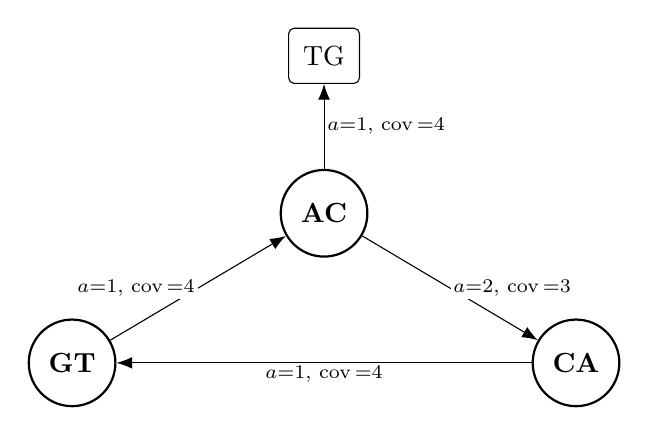
\begin{tikzpicture}[
  hub/.style={draw, thick, circle, minimum size=1.1cm,
              font=\bfseries},
  leaf/.style={draw, rounded corners=2pt, minimum width=0.9cm,
               minimum height=0.7cm},
  every edge/.style={draw, -{Latex[length=2mm]}},
  lbl/.style={font=\scriptsize, fill=white, inner sep=1pt}
]
  \node[hub]  (AC) at (0,0)     {AC};
  \node[hub]  (CA) at (3.2,-1.9){CA};
  \node[hub]  (GT) at (-3.2,-1.9){GT};
  \node[leaf] (TG) at (0,2)     {TG};

  \draw (AC) edge node[lbl, right] {\(a{=}2\), cov\({\,=}3\)} (CA);
  \draw (CA) edge node[lbl, below] {\(a{=}1\), cov\({\,=}4\)} (GT);
  \draw (GT) edge node[lbl, left]  {\(a{=}1\), cov\({\,=}4\)} (AC);
  \draw (AC) edge node[lbl, right] {\(a{=}1\), cov\({\,=}4\)} (TG);
\end{tikzpicture}
\caption{The preference graph of $(\mathtt{AGCT})^5$. An edge
  $w \to c$ means ``$c$'s preferred link sources from $I_w$''. Four
  vertices, four edges, out-degree one everywhere: a pseudoforest with
  exactly one cycle, $\mathtt{AC} \to \mathtt{CA} \to \mathtt{GT} \to
  \mathtt{AC}$, and one pendant.}
\label{fig:prefgraph}
\end{figure}

\subsection{Phase 1: cycle breaking}

Algorithm~\ref{alg:forest} visits names in ascending code order. The
codes here are $\mathtt{AC} = 3$, $\mathtt{CA} = 7$, $\mathtt{GT} = 15$,
$\mathtt{TG} = 19$, so the order is
$\mathtt{AC}, \mathtt{CA}, \mathtt{GT}, \mathtt{TG}$.

\begin{center}
\begin{tabular}{clll}
\toprule
step & name & would set & outcome \\
\midrule
1 & \texttt{AC} & $\mathrm{parent}[\mathtt{AC}] = \mathtt{GT}$ &
  installed (\texttt{GT} has no ancestors yet) \\
2 & \texttt{CA} & $\mathrm{parent}[\mathtt{CA}] = \mathtt{AC}$ &
  installed \\
3 & \texttt{GT} & $\mathrm{parent}[\mathtt{GT}] = \mathtt{CA}$ &
  \textbf{discarded}: $\mathtt{CA} \to \mathtt{AC} \to \mathtt{GT}$ \\
4 & \texttt{TG} & $\mathrm{parent}[\mathtt{TG}] = \mathtt{AC}$ &
  installed \\
\bottomrule
\end{tabular}
\end{center}

At step~3, \texttt{HasAncestor}$(\mathtt{CA}, \mathtt{GT})$ walks
$\mathtt{CA} \to \mathtt{AC} \to \mathtt{GT}$ and finds \texttt{GT}, so
the edge would close the cycle and is dropped. \texttt{GT} keeps its
preferred candidate as a \emph{value} --- it just has no parent, so the
DP will not be able to use it. The trace confirms the forest:

\begin{verbatim}
=== tree-dp forest (src -> dependents) ===
  AC -> CA TG
  GT -> AC
roots: GT
\end{verbatim}

\begin{figure}[h]
\centering
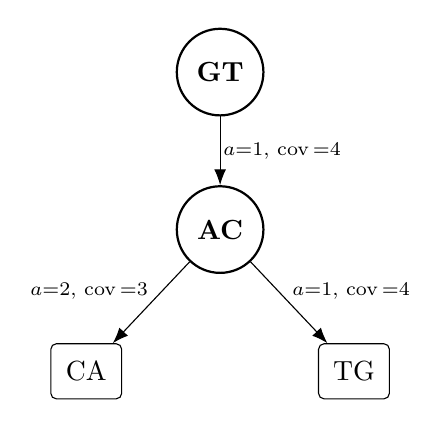
\begin{tikzpicture}[
  hub/.style={draw, thick, circle, minimum size=1.1cm,
              font=\bfseries},
  leaf/.style={draw, rounded corners=2pt, minimum width=0.9cm,
               minimum height=0.7cm},
  every edge/.style={draw, -{Latex[length=2mm]}},
  lbl/.style={font=\scriptsize, fill=white, inner sep=1pt}
]
  \node[hub]  (GT) at (0,2)      {GT};
  \node[hub]  (AC) at (0,0)      {AC};
  \node[leaf] (CA) at (-1.7,-1.8){CA};
  \node[leaf] (TG) at (1.7,-1.8) {TG};

  \draw (GT) edge node[lbl, right]     {\(a{=}1\), cov\({\,=}4\)} (AC);
  \draw (AC) edge node[lbl, above left]{\(a{=}2\), cov\({\,=}3\)} (CA);
  \draw (AC) edge node[lbl, above right]{\(a{=}1\), cov\({\,=}4\)} (TG);
\end{tikzpicture}
\caption{The forest after cycle breaking. One tree, root \texttt{GT}.}
\label{fig:forest}
\end{figure}

\subsection{Phase 1: the DP}

The DP runs bottom-up on Figure~\ref{fig:forest}. Interval sizes are
$\isize(\mathtt{GT}) = 5$, $\isize(\mathtt{AC}) = 5$,
$\isize(\mathtt{CA}) = 4$, $\isize(\mathtt{TG}) = 4$.

\begin{table}[h]
\centering
\caption{The DP table for $(\mathtt{AGCT})^5$. Entries are
  $(\KEEP, \COMP)$ costs with the winner in bold; ``---'' marks an
  unavailable \COMP{} branch.}
\label{tab:dp}
\begin{tabular}{llrrl}
\toprule
node & state & \KEEP{} & \COMP{} & decision \\
\midrule
\texttt{CA} (leaf) & $\mathit{src\_ok} = \mathsf{true}$
  & $4$ & $\mathbf{4 - 3 = 1}$ & \COMP \\
\texttt{CA} (leaf) & $\mathit{src\_ok} = \mathsf{false}$
  & $\mathbf{4}$ & --- & \KEEP \\
\midrule
\texttt{TG} (leaf) & $\mathit{src\_ok} = \mathsf{true}$
  & $4$ & $\mathbf{4 - 4 = 0}$ & \COMP \\
\texttt{TG} (leaf) & $\mathit{src\_ok} = \mathsf{false}$
  & $\mathbf{4}$ & --- & \KEEP \\
\midrule
\texttt{AC} & $\mathit{src\_ok} = \mathsf{true}$
  & $\mathbf{5 + 1 + 0 = 6}$ & $5 - 4 + 4 + 4 = 9$ & \KEEP \\
\midrule
\texttt{GT} (root) & ---
  & $\mathbf{5 + 6 = 11}$ & n/a & \KEEP \\
\bottomrule
\end{tabular}
\end{table}

The middle row is the interesting one and is exactly the comparison the
whole construction exists to make. If \texttt{AC} compresses it saves
its own $4$ ranks, but it must then keep its source ranks alive, which
forbids both children from compressing and costs $1 + 0 \to 4 + 4$, a
net loss of $3$. So \texttt{AC} keeps. The root \texttt{GT} reports
\texttt{comp=n/a} because its preferred source, \texttt{CA}, is a
descendant --- the root rule of \S\ref{sec:dp}. The trace agrees:

\begin{verbatim}
root GT: keep=11 comp=n/a
\end{verbatim}

The DP's value $11$ is the cost of the \emph{tree}, whose four names
hold $5+5+4+4 = 18$ ranks; it saves $18 - 11 = 7$. Adding the three
singleton ranks gives $14$ stored positions after the accept pass. (That
this eventually coincides with the final $|C| = 11$ is a coincidence of
this instance.)

\subsection{Phase 1: accept and leftover}

\texttt{AcceptSubtree} recurses deepest-first from the root, so the
order is \texttt{CA}, \texttt{TG}, \texttt{AC}, \texttt{GT}; only the
first two were chosen:

\begin{verbatim}
[tree-dp] accept chosen...
  ACCEPT CA <- AC add=2 cov=3
  ACCEPT TG <- AC add=1 cov=4
\end{verbatim}

State after the accept pass:
\begin{itemize}
\item removed: ranks $7,8,9$ (of \texttt{CA}) and $17,18,19,20$ (of
  \texttt{TG}); $\mathit{kept} = 21 - 7 = 14$;
\item pinned: \texttt{CA}'s link sources $[3,6)$ and \texttt{TG}'s
  sources $[2,6)$, so ranks $2,3,4,5$ of $I_{\mathtt{AC}}$ carry pins.
\end{itemize}

The leftover pass now considers the two names with no link, \texttt{AC}
and \texttt{GT} (both of size $5$).

\begin{description}
\item[\texttt{AC} gets nothing.] Its two candidates cover
  $\{1,2,3,4\}$ and $\{1,2,3\}$ respectively. Ranks $2,3,4$ are pinned,
  because \texttt{AC}'s own dependents are reading them. Neither
  candidate is available. \emph{The hub is protected from itself}, and
  this happens automatically through the pin counter --- nothing in the
  DP or the accept pass had to arrange it.
\item[\texttt{GT} gets its third-choice link.] Walking the cached list
  in $(\cov \downarrow, a \downarrow)$ order:
  \begin{itemize}
    \item $\cov = 4$, $a = 1$, source $[7,11) \subseteq
      I_{\mathtt{CA}}$: ranks $7,8,9$ were removed, so the source is not
      kept. Rejected by (F2).
    \item $\cov = 3$, $a = 3$, source $[3,6) \subseteq I_{\mathtt{AC}}$:
      source fully kept; covered ranks $11,12,13$ neither removed nor
      pinned. \textbf{Accepted.}
  \end{itemize}
\end{description}

That last acceptance removes three more ranks, bringing $\mathit{kept}$
to $11$. Note that all three accepted links now source from
$I_{\mathtt{AC}}$ --- which is legal precisely because (F2) constrains
sources against \emph{covered} ranks, not against each other
(\texttt{tree\_dp3}, Lemma~5(b)).

\subsection{Phase II and the result}

Phase~II visits the four compressible names, finds every one either
saturated or without a better available candidate, and exits at a fixed
point in one generation having changed nothing.

The final hash table, printed by \texttt{--table}:

\begin{center}
\begin{tabular}{llll}
\toprule
name & code & $H_{\mathrm{offset}}(\mathit{pos}, a, \mathit{num})$ &
$H_{\mathrm{rest}}(\mathit{pos}, \mathit{num})$ \\
\midrule
\texttt{\$\$} &  0 & nil       & $(0,1)$ \\
\texttt{AC}   &  3 & nil       & $(1,5)$ \\
\texttt{C\$}  &  6 & nil       & $(6,1)$ \\
\texttt{CA}   &  7 & $(3,2,3)$ & $(7,1)$ \\
\texttt{GT}   & 15 & $(3,3,3)$ & $(8,2)$ \\
\texttt{T\$}  & 16 & nil       & $(10,1)$ \\
\texttt{TG}   & 19 & $(2,1,4)$ & nil \\
\bottomrule
\end{tabular}
\end{center}

The kept ranks, in rank order, are
$0;\ 1,2,3,4,5;\ 6;\ 10;\ 14,15;\ 16$, so
\[
  C = [\,20,\ 16,\ 12,\ 8,\ 4,\ 0,\ 18,\ 2,\ 5,\ 1,\ 19\,],
  \qquad |C| = 11 .
\]
Every decode can be checked by hand against this array. For
\texttt{TG}, $H_{\mathrm{offset}} = (2,1,4)$ reads
$C[2..5] = 12, 8, 4, 0$ and adds $1 \cdot s = 3$, giving
$15, 11, 7, 3$: the four \texttt{TG} positions. For \texttt{CA},
$(3,2,3)$ reads $C[3..5] = 8, 4, 0$ and adds $6$, giving $14, 10, 6$;
the fourth \texttt{CA} position, $2$, is stored literally at
$C[7]$, which is what $H_{\mathrm{rest}} = (7,1)$ says. For \texttt{GT},
$(3,3,3)$ reads the same three source positions and adds $9$, giving
$17, 13, 9$, with $5$ and $1$ kept at $C[8], C[9]$.

Finally, from \texttt{ilp\_baseline}:
\[
  \text{optimal } |C| = 11
  \quad\text{versus}\quad
  \texttt{greedy}=14,\
  \texttt{dep-order}=11,\
  \texttt{tree-dp}=11 .
\]
\texttt{tree-dp} is optimal here, and the leftover pass was
indispensable: without it the answer would have been $14$.

\section{The isomorphic twin: where cycle breaking costs two positions}
\label{sec:twin}

Now take $T = (\mathtt{ACGT})^5$ --- the same four letters, permuted ---
with the same shape. Again $m = 21$, again seven names, again four
compressible ones of sizes $5, 5, 4, 4$.

\subsection{The two instances are the same problem}

Consider the relabelling
\[
  \mathtt{AC} \mapsto \mathtt{AG},\quad
  \mathtt{CA} \mapsto \mathtt{GA},\quad
  \mathtt{GT} \mapsto \mathtt{CT},\quad
  \mathtt{TG} \mapsto \mathtt{TC}.
\]
Under it, the interval sizes correspond, and --- checked mechanically
over the \emph{full} link universe of both instances, all $15$
candidates each, comparing shifts, coverages, source names, and
source/covered positions relative to their intervals --- the two
candidate sets correspond exactly. As optimization problems in the sense
of \S\ref{sec:setup}, $(\mathtt{AGCT})^5$ and $(\mathtt{ACGT})^5$ under
\texttt{\#.\#} are the same instance with the names renamed. In
particular both have optimum $|C| = 11$.

The same check run over all $24$ permutations $\sigma$ of the alphabet,
comparing $(\sigma_1\sigma_2\sigma_3\sigma_4)^5$ against
$(\mathtt{ACGT})^5$ under the induced relabelling, reports that
\emph{every one} of the $24$ is isomorphic to the reference instance,
and \texttt{ilp\_baseline} gives optimum $11$ for all $24$. Yet:

\begin{center}
\begin{tabular}{lrrrrr}
\toprule
instance & optimum & \texttt{greedy} & \texttt{dep-order} &
\texttt{tree-dp} & \texttt{tree-dp3} \\
\midrule
$(\mathtt{AGCT})^5$ & 11 & 14 & 11 & \textbf{11} & 11 \\
$(\mathtt{ACGT})^5$ & 11 & 14 & 11 & \textbf{13} & 11 \\
\bottomrule
\end{tabular}
\end{center}

and across the whole orbit:

\begin{center}
\small
\begin{tabular}{rrrrr>{\raggedright\arraybackslash}p{4.9cm}}
\toprule
\texttt{tree-dp} & \texttt{tree-dp2} & \texttt{tree-dp3} &
\texttt{dep-order} & \texttt{greedy} & permutations \\
\midrule
$11$ & $11$ & $11$ & $11$ & $14$ &
  \texttt{AGCT ATCG ATGC CGAT CTAG CTGA GTAC GTCA} \\
\addlinespace
$13$ & $13$ & $11$ & $11$ & $14$ & the other sixteen \\
\bottomrule
\end{tabular}
\end{center}

\texttt{greedy}, \texttt{dep-order} and \texttt{tree-dp3} each return the
same value on all $24$ isomorphic instances, as they must if their
answer depends only on the problem. \texttt{tree-dp} and its
Phase-II-less variant \texttt{tree-dp2} split the orbit one third /
two thirds according to how the four gapped $k$-mers happen to sort.

\subsection{What differs}

Only the arithmetic codes, and hence the visit order of
Algorithm~\ref{alg:forest}:
\[
  \underbrace{\mathtt{AC}\,(3) <
  \mathtt{CA}\,(7) < \mathtt{GT}\,(15) < \mathtt{TG}\,(19)}_{(\mathtt{AGCT})^5}
  \qquad\text{versus}\qquad
  \underbrace{\mathtt{AG}\,(4) < \mathtt{CT}\,(10) <
  \mathtt{GA}\,(12) < \mathtt{TC}\,(18)}_{(\mathtt{ACGT})^5} .
\]
Translating the second through the relabelling gives the order
$\mathtt{AC}, \mathtt{GT}, \mathtt{CA}, \mathtt{TG}$ --- the middle two
swapped. That is the entire difference between the two runs.

The consequence is a different edge cut and a different forest shape:

\begin{figure}[h]
\centering
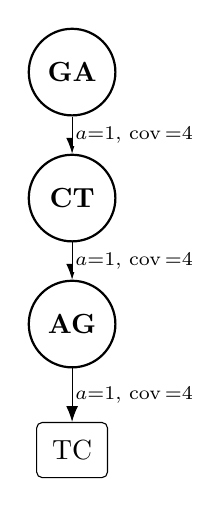
\begin{tikzpicture}[
  hub/.style={draw, thick, circle, minimum size=1.1cm, font=\bfseries},
  leaf/.style={draw, rounded corners=2pt, minimum width=0.9cm,
               minimum height=0.7cm},
  every edge/.style={draw, -{Latex[length=2mm]}},
  lbl/.style={font=\scriptsize, fill=white, inner sep=1pt}
]
  \node[hub]  (GA) at (0,2)     {GA};
  \node[hub]  (CT) at (0,0.4)   {CT};
  \node[hub]  (AG) at (0,-1.2)  {AG};
  \node[leaf] (TC) at (0,-2.8)  {TC};

  \draw (GA) edge node[lbl, right] {\(a{=}1\), cov\({\,=}4\)} (CT);
  \draw (CT) edge node[lbl, right] {\(a{=}1\), cov\({\,=}4\)} (AG);
  \draw (AG) edge node[lbl, right] {\(a{=}1\), cov\({\,=}4\)} (TC);
\end{tikzpicture}
\caption{The forest \texttt{tree-dp} builds on $(\mathtt{ACGT})^5$: a
  path, not a star. The discarded edge is
  $\mathrm{parent}[\mathtt{GA}] = \mathtt{AG}$ (coverage $3$), because
  \texttt{GA} is visited third and by then
  $\mathtt{AG} \to \mathtt{CT} \to \mathtt{GA}$ already exists.}
\label{fig:twinforest}
\end{figure}

\subsection{Why the path loses}

The DP on Figure~\ref{fig:twinforest}:
\begin{align*}
  \mathrm{DP}(\mathtt{TC},\mathsf{true}) &= \min(4,\ 4-4) = 0,
  &\mathrm{DP}(\mathtt{TC},\mathsf{false}) &= 4, \\
  \mathrm{DP}(\mathtt{AG},\mathsf{true}) &= \min(5+0,\ 5-4+4) = 5
  \ \ (\text{tie} \Rightarrow \KEEP),
  &\mathrm{DP}(\mathtt{AG},\mathsf{false}) &= 5+0 = 5, \\
  \mathrm{DP}(\mathtt{CT},\mathsf{true}) &= \min(5+5,\ 5-4+5) = 6
  \ \ (\COMP), \\
  \mathrm{DP}(\mathtt{GA}) &= 4 + 6 = 10 \ \ (\KEEP,\ \texttt{comp=n/a}).
\end{align*}
The trace prints \texttt{root GA: keep=10 comp=n/a}, and the accept pass
takes \texttt{TC} and \texttt{CT}, coverage $4 + 4 = 8$, leaving
$\mathit{kept} = 13$.

Now the leftover pass runs and, unlike in \S\ref{sec:example}, finds
nothing:
\begin{itemize}
\item \texttt{AG}'s candidates cover ranks $\{1,2,3,4\}$ and
  $\{1,2,3\}$; \texttt{TC}'s accepted link sources $[2,6)$, pinning
  $2,3,4,5$. Blocked.
\item \texttt{GA}'s two candidates both cover $\{12,13,14\}$; but
  \texttt{CT} \emph{compressed}, and its link sources $[12,16)$, pinning
  all of $12,13,14,15$. Blocked.
\end{itemize}
Phase~II then confirms a fixed point. Final $|C| = 13$.

The single decision that separates the two runs is at
$\mathrm{DP}(\mathtt{CT})$: on the path, compressing \texttt{CT} is
worth $6$ against $10$, so the DP takes it --- and in doing so pins
$I_{\mathtt{GA}}$ solid, which is what starves the leftover pass. In the
star of Figure~\ref{fig:forest} the corresponding node (\texttt{AC}) is
an internal node with \emph{two} children, so compressing it would cost
two forced \KEEP{}s rather than one; it keeps, and its interval stays
available as a source for the leftover pass to exploit.

\subsection{Two restrictions, interacting}

It would be too simple to blame the cut edge alone. \texttt{tree\_dp3}
\S2.3 analyses this instance and shows that the optimal solution asks
\texttt{CT} to take a link it does \emph{not} prefer --- coverage $3$ at
$a = 3$ sourcing from $I_{\mathtt{AG}}$, rather than its preferred
coverage-$4$ link at $a = 1$ sourcing from $I_{\mathtt{GA}}$ --- because
moving its source off $I_{\mathtt{GA}}$ is what frees \texttt{GA} to
compress in turn. So restriction~(1) of Fact~\ref{fact:loss} binds: no
choice of cut edge lets the \emph{DP} express the optimum, because the
DP only ever offers a name its preferred link.

What saves the successful eight permutations is the pass the DP does not
control. Translating the $(\mathtt{AGCT})^5$ run of \S\ref{sec:example}
through the relabelling, its three accepted links are
\[
  \mathtt{TC} \leftarrow \mathtt{AG}\ (a{=}1,\ \cov 4),\quad
  \mathtt{GA} \leftarrow \mathtt{AG}\ (a{=}2,\ \cov 3),\quad
  \mathtt{CT} \leftarrow \mathtt{AG}\ (a{=}3,\ \cov 3),
\]
which is exactly the optimal triple of \texttt{tree\_dp3} \S2.3 --- and
the third of them is precisely the non-preferred link. The DP supplied
the first two; the \emph{leftover greedy} supplied the third, because
the leftover pass walks the whole cached candidate list and is under no
obligation to take the preferred entry. So the two restrictions
compose as follows.

\begin{remark}
\label{rem:interaction}
On this instance the DP alone can never reach $11$, whatever the cut
(restriction~1). The leftover pass \emph{can} contribute the missing
non-preferred link --- but only if the cut left the relevant interval
unpinned, which is a property of the forest shape (restriction~3).
Under a star, \texttt{AG}'s dependents pin \texttt{AG} but leave
\texttt{CT} free, and the leftover pass closes the gap; under a path,
the DP's decision to compress \texttt{CT} pins all of $I_{\mathtt{GA}}$
and the leftover pass finds nothing. Neither restriction is sufficient
on its own to explain the $13$.
\end{remark}

\texttt{tree-dp3} removes both at once, by re-solving the dependency
cluster $\{\mathtt{AG},\mathtt{CT},\mathtt{GA},\mathtt{TC}\}$ exactly
over the full enumerated universe after Phase~II; it returns $11$ on all
$24$ permutations. See \texttt{tree\_dp3} \S2.3 and \S5.

\section{The smallest counterexample, and what no later pass can fix}
\label{sec:ce}

The second worked instance is
$T = (\mathtt{AC})^6 = \mathtt{ACACACACACAC}$ with $S = \mathtt{\#.\#}$,
$m = 13$. It is analysed in full in \texttt{tree\_dp3} \S2.2
(Counterexample~I); we recall it here because it isolates the cut-edge
restriction more cleanly than \S\ref{sec:twin} does, and because it is
the case \texttt{tree-dp} cannot recover from.

Positions alternate: even positions carry $\mathtt{AA}$, odd positions
carry $\mathtt{CC}$, giving $I_{\mathtt{AA}} = [2,7)$ and
$I_{\mathtt{CC}} = [8,13)$, both of size $5$, plus three singletons.
A link shifts text positions by $3a$, and $\mathtt{AA}$ sits on even
while $\mathtt{CC}$ sits on odd positions, so $a$ must be odd and
$a \ge 3$ overshoots: every link has $a = 1$. The enumerated universe
has exactly two members,
\[
  k_1 : \mathtt{AA} \leftarrow \mathtt{CC},\ \cov = 3,
  \qquad
  k_2 : \mathtt{CC} \leftarrow \mathtt{AA},\ \cov = 4 .
\]
Each is the other's target, so the preference graph is a $2$-cycle, and
the two orientations are \emph{not} worth the same: $k_2$ covers four
ranks, $k_1$ only three. The sources of $k_1$ and $k_2$ each meet the
other's covered set, so by (F2) at most one may be chosen and the
optimum is $|C| = 13 - 4 = 9$, using $k_2$.

Algorithm~\ref{alg:forest} visits $\mathtt{AA}$ (code $2$) before
$\mathtt{CC}$ (code $8$). It installs
$\mathrm{parent}[\mathtt{AA}] = \mathtt{CC}$ and then discards the
reverse edge, which would close the cycle. The forest is the single
edge $\mathtt{CC} \to \mathtt{AA}$ with root $\mathtt{CC}$, and

\[
  \mathrm{DP}(\mathtt{AA},\mathsf{true}) = \min(5,\ 5-3) = 2
  \ \ (\COMP),
  \qquad
  \mathrm{DP}(\mathtt{CC}) = 5 + 2 = 7
  \ \ (\KEEP,\ \texttt{comp=n/a}),
\]
matching the traced \texttt{root CC: keep=7 comp=n/a}. The accept pass
takes $k_1$, and $|C| = 13 - 3 = 10$.

The point is what the cut destroyed. Had the loop installed
$\mathrm{parent}[\mathtt{CC}] = \mathtt{AA}$ instead --- which it would
have, on any instance whose two names sorted the other way --- the tree
would be $\mathtt{AA} \to \mathtt{CC}$, the DP would compute
$\mathrm{DP}(\mathtt{CC},\mathsf{true}) = \min(5, 5-4) = 1$ and
$\mathrm{DP}(\mathtt{AA}) = 5 + 1 = 6$, accept $k_2$, and land on the
optimum $9$. The better of the two orientations was available, it was
better by a whole covered rank, and the algorithm discarded it because
$\mathtt{AA} < \mathtt{CC}$ alphabetically.

Unlike \S\ref{sec:twin}, nothing downstream repairs this. After $k_1$ is
accepted, $\mathtt{AA}$ is saturated and $\mathtt{CC}$'s only candidate
$k_2$ has its source inside the ranks $k_1$ removed, so the leftover
pass and Phase~II both see a fixed point immediately. (\texttt{dep-order}
does reach $9$ here, because its accept order leaves $\mathtt{CC}$ the
first move and its Phase~II retarget finds the coverage-$4$ link; and
\texttt{greedy} gets $10$. No method in the family dominates another.)

The two counterexamples compare as follows.

\begin{center}
\small
\begin{tabular}{p{6.1cm}ll}
\toprule
& $(\mathtt{AC})^6$ & $(\mathtt{ACGT})^5$ \\
\midrule
\texttt{tree-dp} / optimum & $10 / 9$ & $13 / 11$ \\
cut edge is decisive (3) & yes & yes \\
DP can express the optimum & under the other cut & under no cut \\
optimum needs a non-preferred link (1) & no & yes \\
a later pass rescues it & no & under the right cut \\
\bottomrule
\end{tabular}
\end{center}

Restriction~(2) of Fact~\ref{fact:loss} --- one parent per name --- is
not isolated by either instance; it is the hardest of the three to
exhibit at this scale, because it requires a name whose \emph{second}
choice of source would have paid.

\section{Continuity: the walkthrough's running example}
\label{sec:continuity}

For readers coming from \texttt{dep\_order\_walkthrough}, here is
$T = (\mathtt{GCCTTTAAAG})^3$, $S = \mathtt{\#.\#}$, $m = 31$, at
\texttt{7f9127b}.

Nine names, six compressible: $\mathtt{AA}(3)$, $\mathtt{AG}(5)$,
$\mathtt{CT}(6)$, $\mathtt{GC}(5)$, $\mathtt{TA}(6)$, $\mathtt{TT}(3)$.
Preferences:

\begin{center}
\begin{tabular}{lrrll}
\toprule
target & $\cov$ & $a$ & source run & source name \\
\midrule
\texttt{AA} & 3 & 2 & $[19,22)$ & \texttt{GC} \\
\texttt{AG} & 5 & 2 & $[11,16)$ & \texttt{CT} \\
\texttt{TA} & 6 & 1 & $[10,16)$ & \texttt{CT} \\
\texttt{TT} & 3 & 1 & $[19,22)$ & \texttt{GC} \\
\bottomrule
\end{tabular}
\end{center}

\texttt{CT} and \texttt{GC} appear only as sources: they have
\emph{no candidates at all}. The walkthrough describes them as
preferring each other with coverage $2$; since \texttt{kMinCoverage} was
raised to $3$, \texttt{emit\_run\_} discards those links during
enumeration and they no longer exist anywhere in the pipeline.

The rest is straightforward. The preference graph is two disjoint stars
with no cycle, so nothing is cut. The forest is
$\mathtt{CT} \to \{\mathtt{AG}, \mathtt{TA}\}$ and
$\mathtt{GC} \to \{\mathtt{AA}, \mathtt{TT}\}$ with roots \texttt{CT}
and \texttt{GC}; both roots report \texttt{comp=n/a} for the simplest
possible reason, namely that they have no preference to compress with.
All four leaves compress, the DP reports $\mathrm{keep} = 6$ and
$\mathrm{keep} = 5$ for the two roots, the leftover pass finds nothing
(the only names without links are \texttt{CT} and \texttt{GC}, which have
no candidates), and Phase~II is a no-op:
\[
  |C| = 31 - (5 + 6 + 3 + 3) = 14,
\]
which the ILP baseline confirms is optimal. The instance is a clean
illustration of hub/leaf structure and a poor illustration of the
algorithm, which is why \S\ref{sec:example} uses a different one.

\begin{remark}[Recommendation, not an edit]
\label{rem:trim}
\S6 of \texttt{dep\_order\_walkthrough} should be reduced to a short
pointer at this document. Two of its statements are now stale --- the
coverage-$2$ preferences for \texttt{CT} and \texttt{GC}, and the
implied ``source outside $I_c$'' rule that
\S\ref{sec:intra} replaced --- and its Tree-DP figure shows edges that
the current enumerator does not produce. What is worth keeping there is
the construction of the gapped suffix array and the
\texttt{greedy}/\texttt{dep-order} comparison, which this note does not
duplicate. \emph{This edit has not been made.}
\end{remark}

\section{Complexity and practical behaviour}
\label{sec:complexity}

\subsection{Asymptotics}

Let $m$ be the number of ranks, $|\Names|$ the number of compressible
names and $a_{\max}$ the shift ceiling.

\begin{itemize}
\item \textbf{Preference enumeration.} For one interval and one shift,
  the scan is $O(\isize(c))$ lookups plus an
  $O(\isize(c) \log \isize(c))$ sort; the intra-interval splitting is
  linear in the run length. Summed over all intervals and shifts, this
  is $O(a_{\max} \cdot m \log m)$ worst case and $O(a_{\max}\, m)$ in
  practice, since the sort is over short lists. It is done once and
  cached.
\item \textbf{Forest construction.} $O(|\Names| \cdot d)$, where $d$
  bounds the parent-chain depth walked by \texttt{HasAncestor}. Observed
  depths are single digits.
\item \textbf{The DP.} $O(|F|)$ time and memory over forest nodes: each
  of the $2|F|$ states is evaluated once.
\item \textbf{Accept and leftover.} $O(\sum_c \isize(c)) = O(m)$ plus a
  scan of cached candidate lists.
\item \textbf{Phase II.} $O(\text{generations} \times \text{tries}
  \times \text{cost of a retarget})$, with a retarget costing
  $O(\text{covered} + \text{dependents})$. Unbounded in principle;
  bounded in practice by the fixed point after two generations
  (\S\ref{sec:phase2}).
\end{itemize}

\subsection{Measured phase timings}

On \texttt{r300-3000.fasta} ($n = 9{,}000{,}000$), with
\texttt{GCSA\_TIMING=1}:

\begin{table}[h]
\centering
\caption{\texttt{tree-dp} phase timings in milliseconds,
  \texttt{r300-3000.fasta}, $a_{\max}=8$.}
\label{tab:timing}
\begin{tabular}{llrrrrrr}
\toprule
shape & threads & pref & forest & dp & accept & leftover & Phase II \\
\midrule
\texttt{\#\#\#\#\#}      & 1 & $1980$ & $0.3$  & $0.4$  & $1.6$  & $1.0$  & $0.8$ \\
\texttt{\#\#\#\#\#}      & 8 & $579$  & $0.4$  & $0.5$  & $1.8$  & $1.0$  & $0.5$ \\
\texttt{\#\#\#\#.\#\#\#\#} & 1 & $838$  & $15.7$ & $15.7$ & $29.9$ & $26.4$ & $32243$ \\
\texttt{\#\#\#\#.\#\#\#\#} & 8 & $238$  & $20.2$ & $14.5$ & $34.5$ & $25.9$ & $36730$ \\
\bottomrule
\end{tabular}
\end{table}

Three things to read off.

\textbf{Preference enumeration dominates when Phase~II has nothing to
do.} On the contiguous shape it is $99.7\,\%$ of the compression time.
This is the regime the parallelization was built for.

\textbf{Phase~II dominates otherwise.} On the gapped shape it is over
$97\,\%$ of the total, in absolute terms two orders of magnitude more
than everything else combined --- and it is serial. The gapped shape
produces far more intervals with improvable links, and each retarget
walks its dependents. Whole-run speedup from threading is therefore
$3.4\times$ on \texttt{\#\#\#\#\#} but nil on
\texttt{\#\#\#\#.\#\#\#\#} --- the two totals there differ by less than
Phase~II's own run-to-run variance --- even though the parallel section
speeds up by the same factor in both shapes. If \texttt{tree-dp}'s wall
time is ever a problem, Phase~II is the thing to attack.

\textbf{The DP is free.} Forest construction, the DP, the accept pass
and the leftover pass together account for $88$~ms of the gapped-shape
run on a $9$~Mbp input, and $3.3$~ms of the contiguous one: $0.3\,\%$
and $0.2\,\%$ of their totals respectively. Whatever \texttt{tree-dp}
costs, it is not the dynamic program.

\subsection{Parallel speedup}

Preference enumeration scales at $1980 \to 579$~ms
(\texttt{\#\#\#\#\#}) and $838 \to 238$~ms (\texttt{\#\#\#\#.\#\#\#\#})
from one to eight threads: $3.4\times$ and $3.5\times$. The gap from
linear is memory-bound, not lock-bound --- the loop body is a
\texttt{pred\_lexpos\_} chase over two large arrays with no shared
mutable state. The per-root DP parallelizes too, but at $15$~ms of work
there is nothing to win.

Absolute Phase~II times vary by $10$--$20\,\%$ between runs on the same
input; the phase is serial and cache-sensitive. The proportions in
Table~\ref{tab:timing} are stable.

\section{Where \texttt{tree-dp} stands}
\label{sec:empirical}

\subsection{Small instances against the ILP optimum}

\texttt{test\_ilp\_cases.sh} solves ten fixed instances exactly with CBC
over the \emph{full} link universe, so the optimum lower-bounds every
heuristic. Re-run at \texttt{7f9127b}:

\begin{table}[h]
\centering
\caption{Fixed ILP cases. Bold marks a heuristic short of the optimum.}
\label{tab:ilp}
\begin{tabular}{llrrrrrr}
\toprule
instance & shape & opt & \texttt{greedy} & \texttt{dep-order} &
\texttt{tree-dp} & \texttt{tree-dp2} & \texttt{tree-dp3} \\
\midrule
note ($n{=}40$)         & \texttt{\#.\#}    & 26 & 26 & 26 & 26 & 26 & 26 \\
$(\mathtt{GCCTTTAAAG})^3$ & \texttt{\#.\#}  & 14 & 14 & 14 & 14 & 14 & 14 \\
$(\mathtt{AC})^6$       & \texttt{\#.\#}    &  9 & \textbf{10} & 9 & \textbf{10} & \textbf{10} & 9 \\
$(\mathtt{AGCT})^5$     & \texttt{\#.\#}    & 11 & \textbf{14} & 11 & 11 & 11 & 11 \\
$(\mathtt{ACGT})^5$     & \texttt{\#.\#}    & 11 & \textbf{14} & 11 & \textbf{13} & \textbf{13} & 11 \\
\texttt{GGGCGGCGGC}     & \texttt{\#\#}     & 11 & 11 & 11 & 11 & 11 & 11 \\
note ($n{=}40$)         & \texttt{\#\#.\#\#}& 35 & 35 & 35 & 35 & 35 & 35 \\
note ($n{=}40$)         & \texttt{\#\#}     & 19 & \textbf{20} & \textbf{20} & \textbf{20} & \textbf{20} & \textbf{20} \\
$\mathtt{A}^{16}$       & \texttt{\#.\#}    & 11 & 11 & 11 & 11 & 11 & 11 \\
$(\mathtt{ACGT})^7$     & \texttt{\#\#.\#}  & 17 & 17 & 17 & 17 & 17 & 17 \\
$(\mathtt{GCCTTTAAAG})^4$& \texttt{\#..\#}  & 22 & \textbf{25} & \textbf{27} & \textbf{27} & \textbf{27} & 22 \\
\bottomrule
\end{tabular}
\end{table}

\texttt{tree-dp} attains the optimum on $7$ of the $11$ rows (the
$(\mathtt{AGCT})^5$ row was added for this note; the script's own ten
give $6$). Where it misses it misses by $1$, $2$, $1$ and $5$. Two of
the four misses are the counterexamples of \S\ref{sec:twin} and
\S\ref{sec:ce}; the note-\texttt{\#\#} row is missed by every heuristic,
including \texttt{tree-dp3}.

\subsection{The 139-configuration suite}

\texttt{compare\_algos} builds $139$ synthetic repeat configurations ---
motif repeats, sparse insertions, mixed structures --- and runs all five
algorithms on each. Totals of $|C|$ over the whole suite, from the
\texttt{7f9127b} build:

\begin{table}[h]
\centering
\caption{Suite totals, $139$ configurations, no correctness failures.}
\label{tab:suite}
\begin{tabular}{lrrrrr}
\toprule
$a_{\max}$ & \texttt{greedy} & \texttt{dep-order} & \texttt{tree-dp} &
\texttt{tree-dp2} & \texttt{tree-dp3} \\
\midrule
$8$  & $259518$ & $252357$ & $252397$ & $256197$ & $252394$ \\
$16$ & $255785$ & $252175$ & $252329$ & $255370$ & $213078$ \\
\bottomrule
\end{tabular}
\end{table}

Reading the default row ($a_{\max} = 8$):

\begin{itemize}
\item \texttt{tree-dp} beats \texttt{greedy} by $2.74\,\%$. That is the
  headline number for the algorithm.
\item \texttt{tree-dp} versus \texttt{tree-dp2} --- the same algorithm
  with Phase~II disabled --- is $252397$ against $256197$. \textbf{Phase
  II is worth $3800$ positions, $1.5\,\%$}, more than the gap between
  \texttt{tree-dp} and \texttt{greedy} is worth over \texttt{dep-order}.
  The retarget loop is not a polish step.
\item \texttt{tree-dp} versus \texttt{dep-order} is $252397$ against
  $252357$: \texttt{tree-dp} is $40$ positions ($0.016\,\%$)
  \emph{worse} suite-wide. The forest DP's global reasoning about hubs
  does not, on this suite, pay for the preference and cut-edge
  restrictions it imposes. Both algorithms share Phase~II, so the
  comparison isolates Phase~I, and Phase~I is roughly a wash.
\item \texttt{tree-dp3}, which re-solves clusters exactly on top of the
  same Phase~II, lands at $252394$ --- three positions better than
  \texttt{tree-dp}. At $a_{\max} = 8$ the candidate universe, not the
  neighbourhood size, is what binds.
\end{itemize}

Reading the $a_{\max} = 16$ row: \texttt{tree-dp} barely moves
($252397 \to 252329$, $0.03\,\%$) while \texttt{tree-dp3} drops by
$15.5\,\%$. This is the quantitative form of the remark in
\S\ref{sec:enumerate}: enlarging the candidate universe is worthless to
an algorithm that only ever looks at one candidate per name.

\subsection{Summary of the empirical picture}

\texttt{tree-dp} is a solid, fast, deterministic heuristic that is
optimal on most small instances and $2.7\,\%$ better than \texttt{greedy}
on the suite. It is not better than \texttt{dep-order}, and most of what
separates both from \texttt{greedy} is Phase~II, which they share. The
forest DP's contribution is real but small, and it is bounded above by
the three restrictions of Fact~\ref{fact:loss} --- which is what motivated
\texttt{tree-dp3}.

\section{Discussion}
\label{sec:discussion}

\paragraph{What the DP buys.}
The pseudoforest property (Corollary~\ref{cor:pseudoforest}) is a real
structural gift: it turns an NP-hard packing problem into a linear-time
tree DP. The DP then answers a question no greedy can: \emph{is this hub
worth more as a source than as a target?} On $(\mathtt{AGCT})^5$ it
answers correctly ($6$ against $9$), keeps \texttt{AC} free, and reaches
the optimum where \texttt{greedy} loses three positions.

\paragraph{What it costs.}
The gift is paid for by three restrictions, and
\S\ref{sec:twin}--\S\ref{sec:ce} show two of them binding on instances
of thirteen and twenty-one ranks. The most uncomfortable is
Fact~\ref{fact:order}: on a cycle, the algorithm's answer depends on the
alphabetical order of $k$-mer names. It is deterministic --- and the
implementation goes to some trouble to keep it deterministic under
parallelism --- but determinism here means only that the same arbitrary
choice is made every time.

\paragraph{An obvious improvement that is not obviously enough.}
Cutting the \emph{minimum-coverage} edge of each cycle instead of the
last-visited one would be a two-line change, and it would fix
$(\mathtt{AC})^6$: the cycle's two edges carry coverage $3$ and $4$, and
dropping the cheaper one leaves exactly the orientation that reaches
$9$. It would \emph{not} fix $(\mathtt{ACGT})^5$, whose cycle carries
coverages $4, 4, 3$ --- the minimum-coverage edge is the one the current
rule already discards, so the heuristic changes nothing there. That is
the general problem with edge-local repairs: the value of an edge to the
DP is not its coverage but the difference it makes to the subtree costs,
which is not known before the DP runs.

The principled version --- try all $\nu$ cuts of each cycle and keep the
best --- costs a factor $\nu$ on cycle components only, which is
probably affordable. But it raises the question of what ``best'' means,
and the measured answer is discouraging. The two forests of
\S\ref{sec:twin} report DP costs of $10$ (the path) and $11$ (the star):
the path is the better forest \emph{by the DP's own objective} and the
worse one by two positions in the final answer, because the DP objective
cannot see that the star leaves an interval unpinned for the leftover
pass to exploit. Selecting cuts by DP value would have picked the wrong
forest here. A correct rule would have to score each cut by running the
rest of the pipeline, which is no longer a two-line change.
\texttt{tree-dp3} instead lifts all three restrictions locally, after
the fact, and gets $15.5\,\%$ at $a_{\max} = 16$.

\begin{remark}[Measured, after this note was drafted]
\label{rem:dp4}
A variant implementing exactly the minimum-coverage repair
(\texttt{tree-dp4}, added at \texttt{2995a80}, after the
\texttt{7f9127b} snapshot this note documents; plain \texttt{tree-dp} is
unchanged there) behaves precisely as the two paragraphs above predict,
in both directions. On $(\mathtt{AC})^6$ it returns the optimum $9$
instead of $10$. On the $(\mathtt{ACGT})^5$ orbit it returns $13$ on
\emph{all $24$} permutations --- so it is now order-independent, which
is progress, but it has given up the eight permutations on which plain
\texttt{tree-dp} reached $11$. Preferring the higher-coverage edge
converts the star of Figure~\ref{fig:forest} into the path of
Figure~\ref{fig:twinforest}, which is the better forest by the DP's
objective and the worse one by two positions after the leftover pass
runs. Edge-local repair of the cut is a genuine improvement on some
instances and a genuine regression on others, for the reason given
above: coverage is not the quantity that matters.
\end{remark}

\paragraph{The leftover pass deserves better billing.}
It is named as if it handled stragglers, but Fact~\ref{fact:intra-dp}
shows it is structurally responsible for \emph{all} intra-interval
links, and \S\ref{sec:example} shows it contributing $30\,\%$ of the
compression on an instance where the DP itself did well. On
$\mathtt{A}^{16}$ it does everything. A reasonable reading of
Algorithm~\ref{alg:treedp} is that \texttt{tree-dp} has two heuristics,
one exact-on-a-forest and one greedy, and that the second is not a
fallback.

\paragraph{Where the time goes.}
Table~\ref{tab:timing} is unambiguous: on a gapped shape at $9$~Mbp,
Phase~II is $97\,\%$ of the work and the entire forest machinery is
$0.3\,\%$. Any future effort spent making the DP faster is misdirected;
any spent parallelizing or pruning the retarget loop is not.

\end{document}
